\documentclass[11pt]{article}
\usepackage[margin=1in]{geometry}
\usepackage{amsmath, amssymb, amsthm}
\usepackage{graphicx}
\usepackage{enumitem}
\usepackage{tikz}
\usetikzlibrary{calc}
\usepackage{hyperref}
\usetikzlibrary{shapes,arrows,positioning,shapes.geometric}

\title{Technical Summary: Deterministic Online Bipartite Edge Coloring}
\author{Team 70 / Ali Ahsan, Hamza Raza}
\date{\today}

\begin{document}
\maketitle

\section{Problem and Contribution}
\textbf{Problem Statement:}  
The paper addresses the \emph{online edge coloring} problem in bipartite graphs. In this setting, the graph’s edges are revealed sequentially, and an algorithm must assign a color to each edge immediately upon arrival. The coloring must be proper (no two adjacent edges share the same color). While Kőnig’s theorem guarantees that an optimal offline coloring of a bipartite graph requires at most $\Delta$ colors (where $\Delta$ is the maximum degree), the online constraint makes it challenging to match this bound.

\textbf{Main Contribution:}  
The authors present a \emph{deterministic} online algorithm that achieves a competitive ratio close to the optimal number of colors. Unlike randomized approaches, which may only guarantee good performance in expectation, the deterministic algorithm provides worst-case guarantees. The novelty lies in how the algorithm adapts to the online arrival of edges, ensuring that each decision is made with provable bounds on the total number of colors used.

\section{Algorithmic Description}
\textbf{Input and Output:}  
\begin{itemize}[noitemsep]
    \item \textbf{Input:} A bipartite graph \(G=(U,V,E)\) with edges arriving one-by-one in an online fashion.
    \item \textbf{Output:} An assignment of colors to each edge such that no two edges sharing a vertex receive the same color.
\end{itemize}

\textbf{High-Level Idea:}  
The algorithm maintains a set of \emph{available colors} for each vertex, updating these sets as new edges arrive. When an edge \((u,v)\) is revealed, the algorithm:
\begin{enumerate}[noitemsep]
    \item Determines the intersection of the available color sets for vertices \(u\) and \(v\).
    \item Assigns the smallest available color (according to a fixed order) from this intersection.
    \item Updates the available color sets for both \(u\) and \(v\), ensuring future edges are assigned colors that do not conflict.
\end{enumerate}

\subsection*{Edge Assignment Diagram}
The diagram below illustrates two vertices \(u\) and \(v\) with their available color sets. When an edge arrives between them, the intersection of these sets is highlighted (in red), and the smallest color from the intersection is chosen and assigned.

\begin{center}
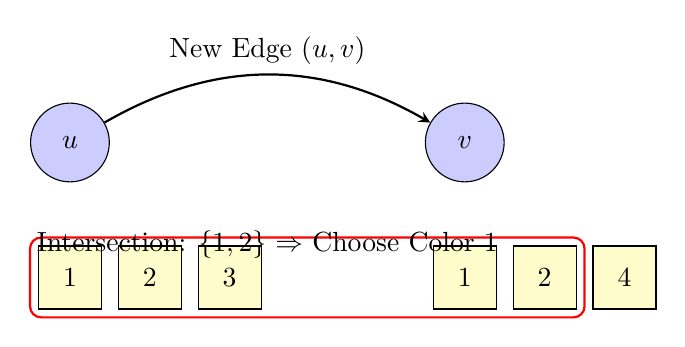
\begin{tikzpicture}[node distance=1.5cm, auto]
    % Define styles
    \tikzstyle{vertex} = [circle, draw, fill=blue!20, minimum size=1cm]
    \tikzstyle{box} = [rectangle, draw, fill=yellow!20, minimum size=0.8cm]
    \tikzstyle{arrow} = [->, >=stealth, thick]
    
    % Draw vertices
    \node[vertex] (u) {\(u\)};
    \node[vertex, right=4cm of u] (v) {\(v\)};
    
    % Draw available color sets below each vertex
    \node[box, below=0.8cm of u] (u1) {1};
    \node[box, right=0.2cm of u1] (u2) {2};
    \node[box, right=0.2cm of u2] (u3) {3};
    \node[box, below=0.8cm of v] (v1) {1};
    \node[box, right=0.2cm of v1] (v2) {2};
    \node[box, right=0.2cm of v2] (v3) {4};
    
    % Highlight the intersection of available colors (common colors: 1 and 2)
    \draw[red, thick, rounded corners] ($(u1.north west) + (-0.1,0.1)$) rectangle ($(v2.south east) + (0.1,-0.1)$);
    
    % Draw the arriving edge
    \draw[arrow, thick, bend left] (u) to node[midway, above] {New Edge \((u,v)\)} (v);
    \newline;
    % Annotation for the chosen color
    \node[below=1cm of $(u)!0.5!(v)$] {Intersection: \(\{1,2\}\) $\Rightarrow$ Choose Color 1};
\end{tikzpicture}
\end{center}

\subsection*{Algorithm Flowchart}
The flowchart below outlines the step-by-step process of the algorithm:
\begin{enumerate}[noitemsep]
    \item \textbf{Edge Arrival:} An edge \((u,v)\) arrives.
    \item \textbf{Compute Intersection:} Compute the intersection of available colors for \(u\) and \(v\).
    \item \textbf{Select Color:} Choose the smallest color from the intersection.
    \item \textbf{Assign \& Update:} Assign this color to the edge and update both vertices’ available color sets.
\end{enumerate}

\begin{center}
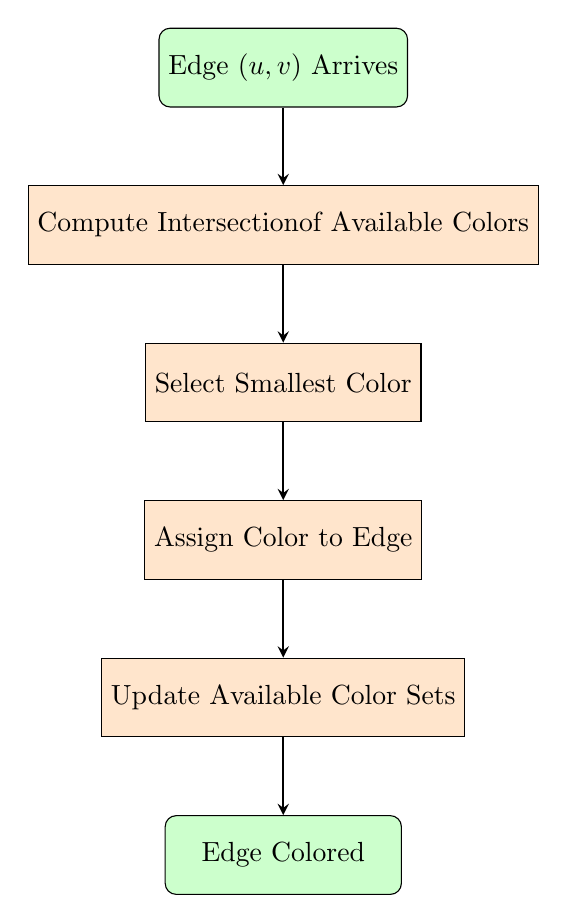
\begin{tikzpicture}[node distance=2cm, auto]
    % Define block styles
    \tikzstyle{startstop} = [rectangle, rounded corners, minimum width=3cm, minimum height=1cm, text centered, draw=black, fill=green!20]
    \tikzstyle{process} = [rectangle, minimum width=3cm, minimum height=1cm, text centered, draw=black, fill=orange!20]
    \tikzstyle{arrow} = [thick,->,>=stealth]

    % Nodes
    \node (start) [startstop] {Edge \((u,v)\) Arrives};
    \node (intersect) [process, below of=start] {Compute Intersection\\of Available Colors};
    \node (select) [process, below of=intersect] {Select Smallest Color};
    \node (assign) [process, below of=select] {Assign Color to Edge};
    \node (update) [process, below of=assign] {Update Available Color Sets};
    \node (stop) [startstop, below of=update] {Edge Colored};

    % Arrows between nodes
    \draw [arrow] (start) -- (intersect);
    \draw [arrow] (intersect) -- (select);
    \draw [arrow] (select) -- (assign);
    \draw [arrow] (assign) -- (update);
    \draw [arrow] (update) -- (stop);
\end{tikzpicture}
\end{center}

\section{Comparison with Existing Approaches}
\textbf{Existing Work:}  
Previous algorithms for online edge coloring include both randomized methods and simpler deterministic greedy approaches. Randomized algorithms can sometimes achieve near-optimal performance in expectation but lack strong worst-case guarantees. Greedy methods, on the other hand, tend to be simple but may use significantly more than \(\Delta\) colors in adversarial scenarios.

\textbf{Novelty and Advantages:}  
The proposed deterministic algorithm is novel because it:
\begin{itemize}[noitemsep]
    \item Provides worst-case performance guarantees without relying on randomness.
    \item Uses a more sophisticated approach to manage available color sets and updates, reducing the risk of “color exhaustion” at any vertex.
    \item Balances the trade-off between immediate decision-making and long-term performance, which is critical in online settings.
\end{itemize}

\section{Data Structures and Techniques}
\textbf{Data Structures:}
\begin{itemize}[noitemsep]
    \item \textbf{Color Availability Lists:} Arrays or bit vectors for each vertex that track which colors are still available.
    \item \textbf{Adjacency Lists:} To store the graph structure and quickly access neighbors when updating available colors.
\end{itemize}

\textbf{Techniques:}
\begin{itemize}[noitemsep]
    \item \textbf{Greedy Selection:} Choosing the smallest available color from the intersection of the two vertices’ available color sets.
    \item \textbf{Potential Function Analysis:} Used in the theoretical analysis to guarantee that the number of colors used does not exceed the bound by too large a factor relative to \(\Delta\).
    \item \textbf{Online Algorithm Design:} Strategies for making irrevocable decisions based on the current state and limited future knowledge.
\end{itemize}

\section{Implementation Outlook and Anticipated Challenges}
\textbf{Technical Challenges:}
\begin{itemize}[noitemsep]
    \item \textbf{Dynamic Updates:} Efficiently updating the available color sets in real time as new edges are added, especially in graphs with high vertex degrees.
    \item \textbf{Scalability:} Ensuring that the algorithm remains efficient with large input sizes. This includes managing memory usage for the color availability data structures.
    \item \textbf{Edge Cases:} Handling adversarial edge sequences that may try to force the algorithm into using suboptimal color choices.
    \item \textbf{Numerical Precision:} While less of a concern in combinatorial problems, careful bookkeeping is needed when indexing and managing color sets.
\end{itemize}

\textbf{Implementation Strategy:}  
To address these challenges, we plan to:
\begin{itemize}[noitemsep]
    \item Optimize the data structures using arrays or bit masks for fast bitwise operations.
    \item Use rigorous unit testing to cover worst-case scenarios and adversarial inputs.
    \item Profile the implementation on synthetic datasets that mimic worst-case inputs to ensure the algorithm’s performance aligns with theoretical guarantees.
\end{itemize}




\end{document}
